
\begin{figure}[!bt]
\centering
\begin{tabular}{@{}c@{}}	
\subfloat[Typical client device current consumption for a complete LoRaWAN transmission. The device is powered at $3V$.]{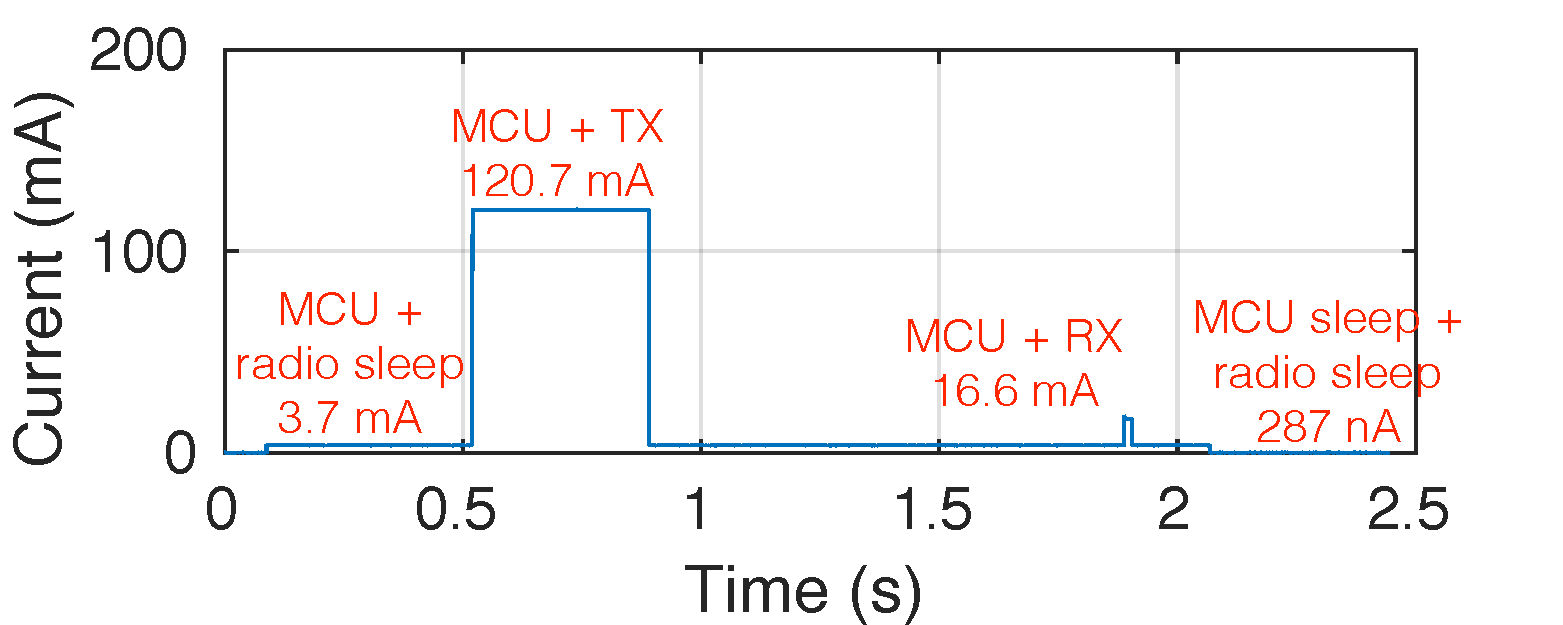
\includegraphics[width=0.36\textwidth]{figures/bug_power_trace_annotated}
\label{fig:power-trace}}\\
\hspace*{0.1in}
\subfloat[Estimated lifetime of a client device powered by two AA batteries sending 36 byte packets at various data rates based on the energy profile.]{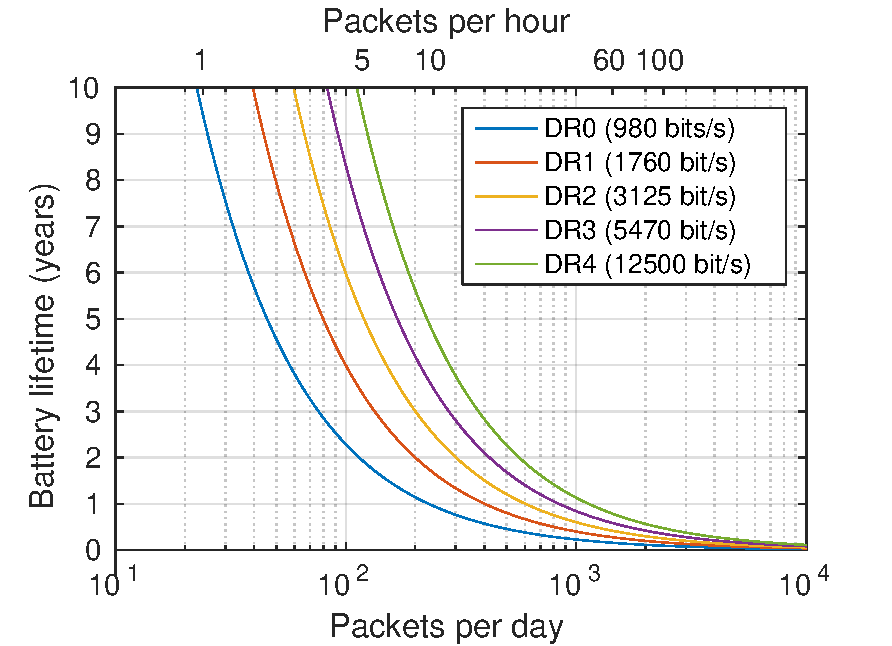
\includegraphics[width=0.36\textwidth]{figures/LoRaBug_AA_lifetime_semilog}
\label{fig:lifetime-estimates}}
\end{tabular}
\vspace*{-0.1in}
\caption{Power statistics}
\compactimg
\end{figure}

\section{Results}
\label{sec:eval}

%{\color{blue} }
%We implemented our system using 8 LPWAN boards as base stations distributed across a university campus.  We used a Semtech SX1276 LoRaWAN transmitter as the client device. We use Charm as the software platform at the backend to support backhaul. 

We evaluate Charm both through proof-of-concept experiments and large-scale
trace-driven simulations. We perform our experiments in various indoors and
outdoors environments across the campus.

\subsection{Role of Transmission Rates on Battery Life}
\label{sec:energy-savings}

\begin{figure}[!htb]
\centering
\compactimg
\subfloat[Success rate for bi-directional packet exchange between client device and gateway]{
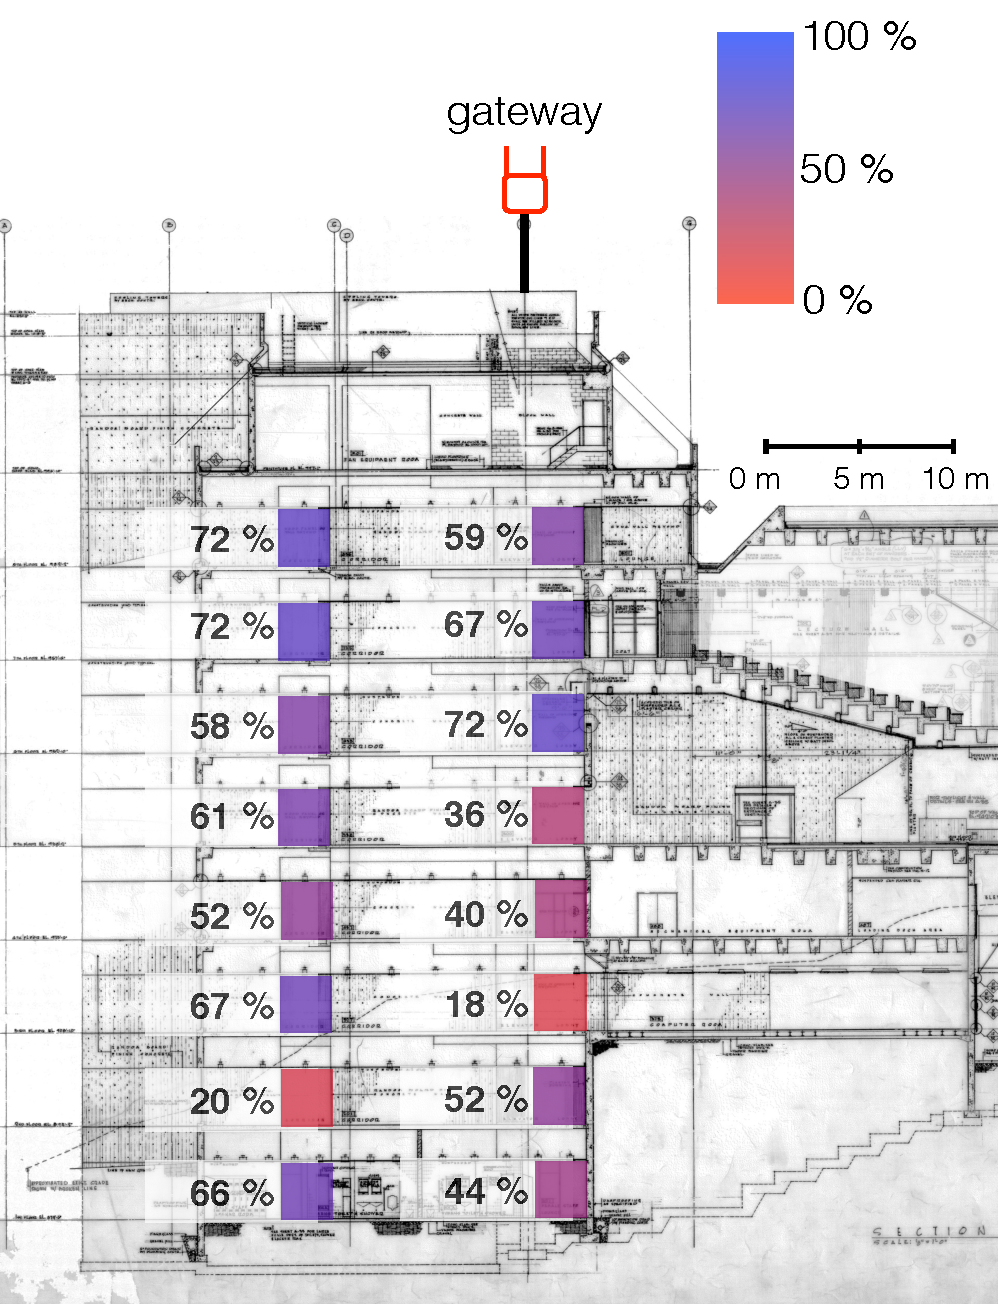
\includegraphics[width=0.45\columnwidth]{figures/penetration_wean_success_cropped}
\label{fig:pen-wean-success}}
\hfill
\subfloat[RSSI at the gateway for successful transfers]{
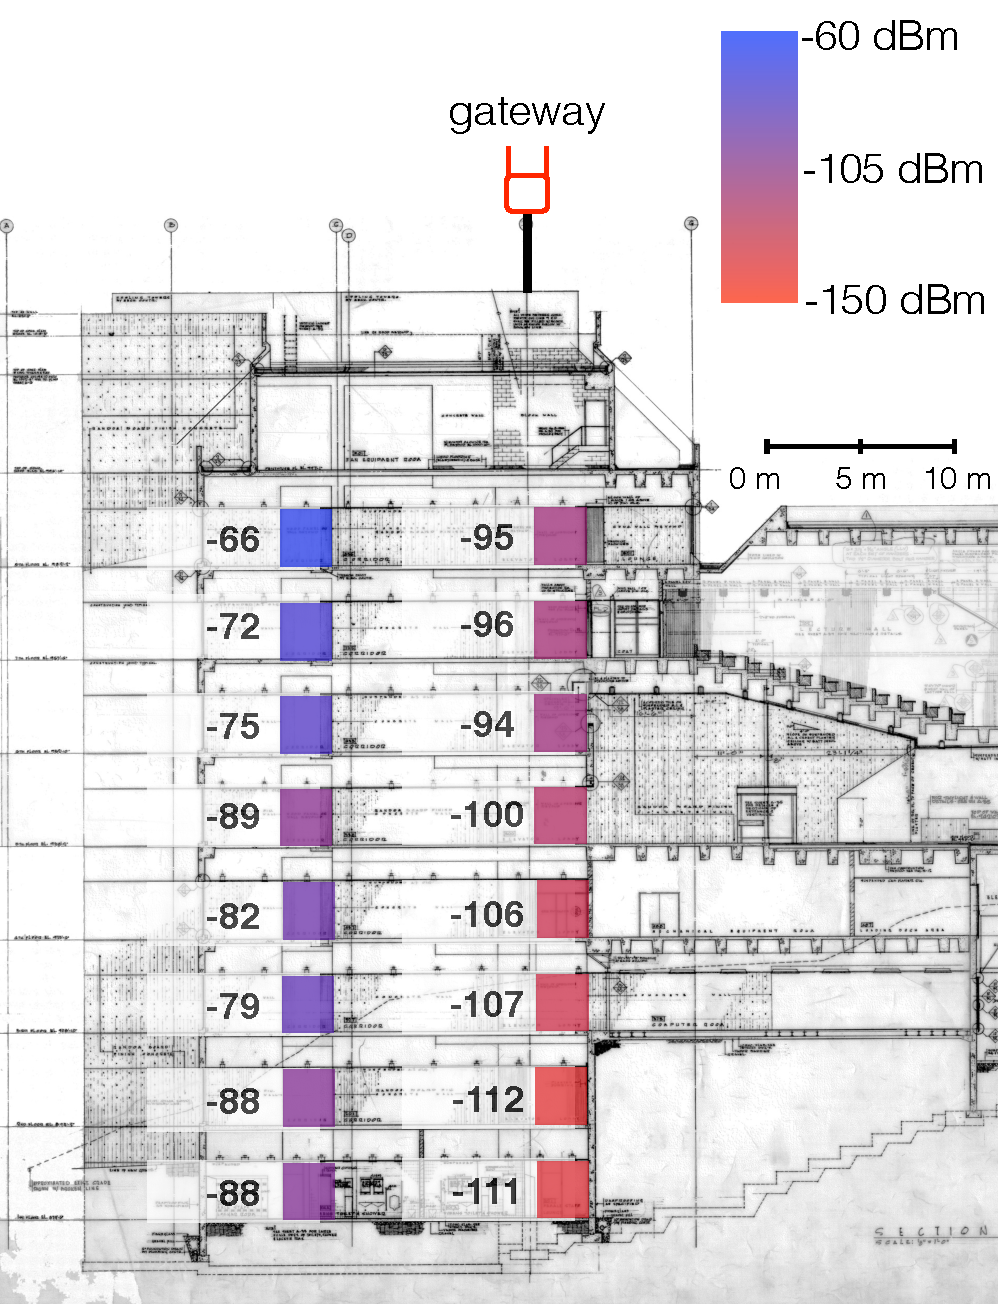
\includegraphics[width=0.45\columnwidth]{figures/penetration_wean_rssi_cropped}
\label{fig:pen-wean-rssi}}
\vspace{-10pt}
\caption{RF signal penetration experiments in a large poured-concrete building}
\label{fig:penetration-test}
\vspace{-10pt}
\end{figure}

\begin{figure*}[!b]
\centering
\subfloat[Local detection capacity at gateways for low SNRs]{
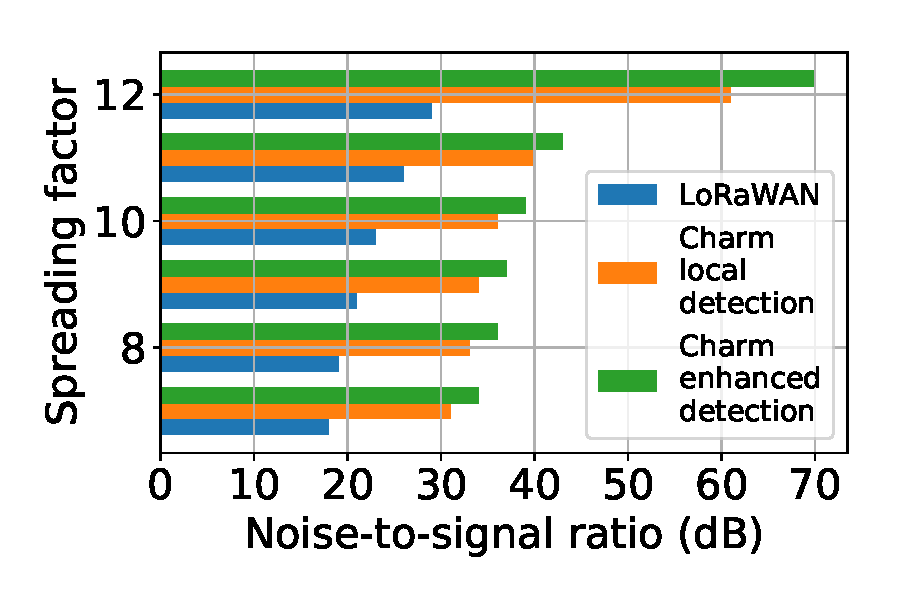
\includegraphics[height=3.5cm]{figures/local_detection_limits}
\label{fig:local-detection}}
\hfill
\subfloat[Diversity gain]{
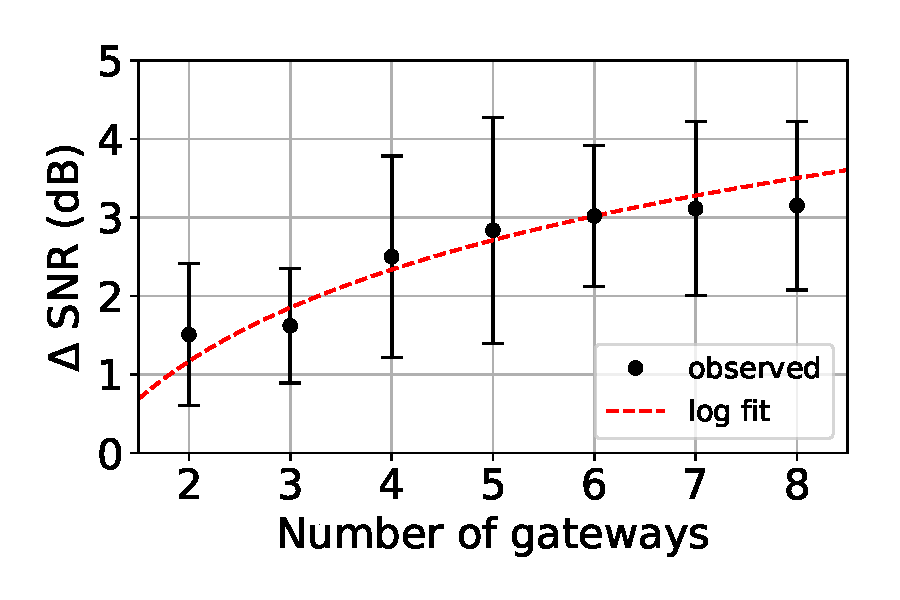
\includegraphics[height=3.5cm]{figures/diversity_gain}
\label{fig:diversity-gain}}
\hfill
\subfloat[Increase in battery life]{
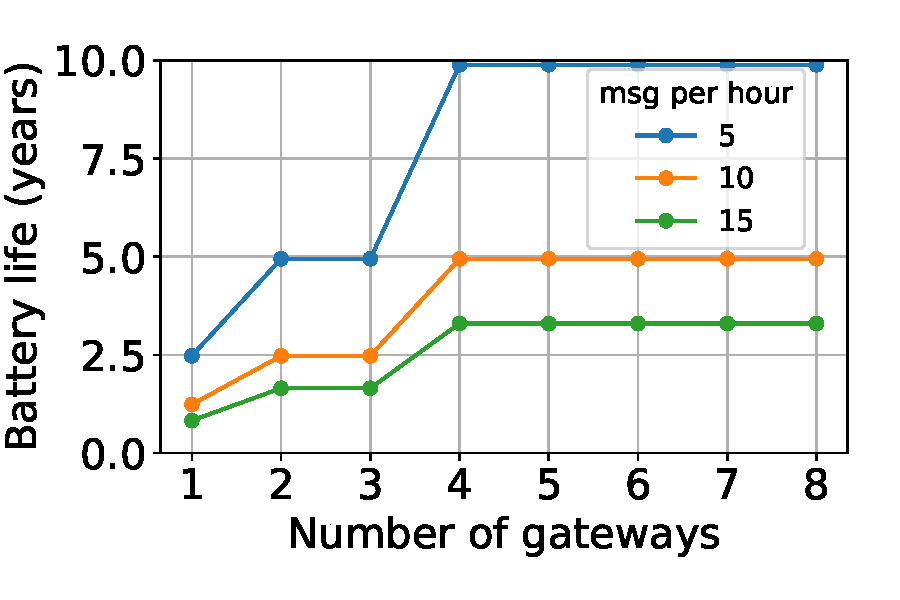
\includegraphics[height=3.5cm]{figures/diversity_battery}
\label{fig:diversity-battery}}
\compactimg
\caption{Results}
\label{fig:results}
\compactimg
\end{figure*}

We study the energy profile of a typical battery-operated LoRaWAN client, as
in \figref{power-trace}. The device performs some local computation, sends a
LoRa message, waits for an acknowledgement and then goes to low-power sleep
mode. The radio transmission consumes the highest amount of energy ($=
\text{area under the curve} \times \text{voltage}$) by a large margin. Thus,
any optimization to battery life must focus on reducing the energy of
transmissions.

Two parameters affect the energy consumed by transmissions: (1) transmit power
and (2) transmit time. Using the currently available LoRa radio chipsets
(Semtech SX1272 and SX1276), we've observed that the transmit power does not
significantly change the power drawn from the battery during transmission. Any
optimization will thus have to focus on reducing the transmit time. The
transmit time is determined by the data rate and the amount of data to send.
We do not control the amount of data generated by client devices and thus,
improving the data rate would provide the largest improvements.

\figref{lifetime-estimates} shows the estimated battery life of a client
device if it were to communicate with different data rates. Wireless systems
try to communicate at the highest data rate that does not cause too many
errors. In the case of LoRa devices, switching to a slower data rate increases
the spreading factor,  which have better sensitivity on the receiver. Thus,
LoRa devices communicating at the highest spreading factors (and
correspondingly using the lowest data rates) can communicate at much longer
range and with higher reliability. The downside is a significant increase in
their transmission time which severely affects battery life. This demonstrates
that Charm can significantly improve battery life should it allow clients to
transmit at higher data rates.

Charm can not only increase range but also increase coverage in urban
scenarios with lots of obstructions and devices deep inside buildings.
\figref{penetration-test} shows a penetration test experiment inside an
on-campus poured-concrete building. Despite a gateway being placed on the roof
of the building, we observe the received signal strength to vary as much as 46
dBm at various locations inside the building. A number of client devices, deep
inside structure, would have been forced to use the the slowest data rate but
can now benefit from Charm.

\subsection{Local detection algorithm}
\label{sec:local-detection-eval}

We performed trace-driven simulation to demonstrate the increase in detection
capability of LoRa packets under noise. To perform this experiment, we collect
data at different spreading factors at high SNRs. We then measure the signal
power and progressively increase additive white Gaussian noise in the signal.
At every dB of decrease in SNR, we test the state-of-the-art LoRaWAN decoding
algorithm against Charm's local and enhanced detection algorithm, where the
former uses the preamble alone and the latter uses both preamble and data in
its optimization.

The results in \figref{local-detection} show that Charm's local detection
algorithm far outperforms the LoRaWAN detection algorithm for detection of the
packet. Further, Charm's enhanced algorithm outperforms Charm's local
detection algorithm by up to 10 dB, as it uses data symbols in addition to the
preamble, improving performance. This demonstrates the value of using data
symbols to better optimize packet detection, particularly in noisy settings.
Our results also reveal a 33\% increase in the negative SNR under which a
packet can be detected, when compared to LoRaWAN -- a gain of between 16-30
dB. To put this in perspective, this is equivalent boost in SNR by coherent
combining of between 40-1000 gateways. Said differently, Charm can even detect
packets that can only be decoded by coherently combining signals from at least
40 gateways that receive the same signal at a similar level of noise.

\subsection{Diversity gain}
\label{sec:diversity-gain-eval}

Next, we evaluate the  gain introduced by Charm in SNR when coherently
combining the multiple transmissions from geographically diverse receivers at
a central server. These benchmarks are completed on a testbed covering 0.6
sq.km. using an ensemble of 8 user-deployed gateways equipped with our custom
LPRAN hardware. This testbed spans multiple buildings and open spaces between
them, and is supposed to emulate a dense urban deployment. We measure the mean
and standard deviation in SNR improvement as a function of number of gateways
across experiments.

Our results reveal remarkable SNR improvements, which as expected improves
steadily with an increasing number of gateways as depicted in Figure
\ref{fig:diversity-gain}, for clients in different locations across multiple
spreading factors. We note that the SNR gain improvement is logarithmic given
that it is measured in dB (a log-scale). Across experiments, Charm gave an
average observable improvement of 1 dB with the addition of each new receiver.
This improvement is valuable, given that every 3 dB of gain allows us to use
the next spreading factor. Any increase in spreading factor halves the
transmission air time and the resulting energy expenditure.
\figref{diversity-battery} depicts the improvement in battery life of an
indoor LoRaWAN client with an increasing number of gateways collaborating to
decode its signal. We observe that the battery life for a device transmitting
5 messages per hour at SF11 improves from 2.5 years to 10 years (SF9) with 4
or more collaborating gateways


\subsection{Range Improvement for Indoor User-Deployed Gateways}

\begin{table}[h]
\centering
\begin{tabular}{r|c|c|}
\cline{2-3}
\multicolumn{1}{l|}{}            & SF7            & SF10           \\ \hline
\multicolumn{1}{|r|}{LoRa}       & \textless60 m  & \textless60 m  \\ \hline
\multicolumn{1}{|r|}{4 gateways} & \textless60 m  & \textless100 m \\ \hline
\multicolumn{1}{|r|}{8 gateways} & \textless200 m & \textless200 m \\ \hline
\end{tabular}
\caption{Range in congested indoor urban settings}
\label{tab:range}
\compactimg
\compactimg
\end{table}

\begin{figure*}[hb]
\centering
\subfloat[Dense cells]{
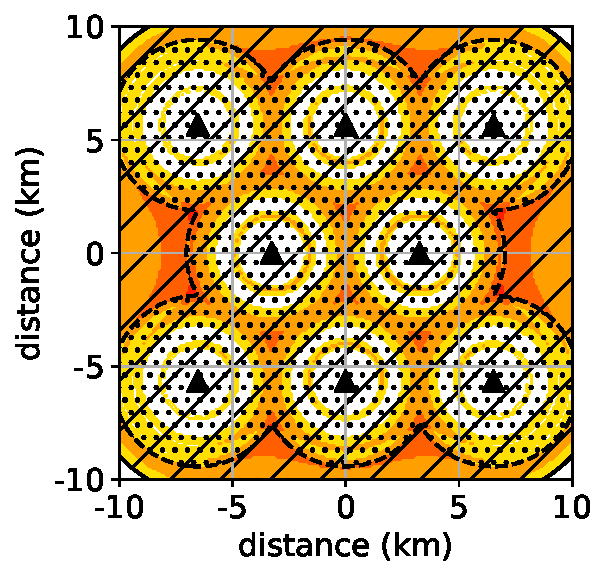
\includegraphics[height=3.25cm]{figures/dense_IncreaseHeatmap}
\label{fig:dense-improvement}}
\hfill
\subfloat[Sparse cells]{
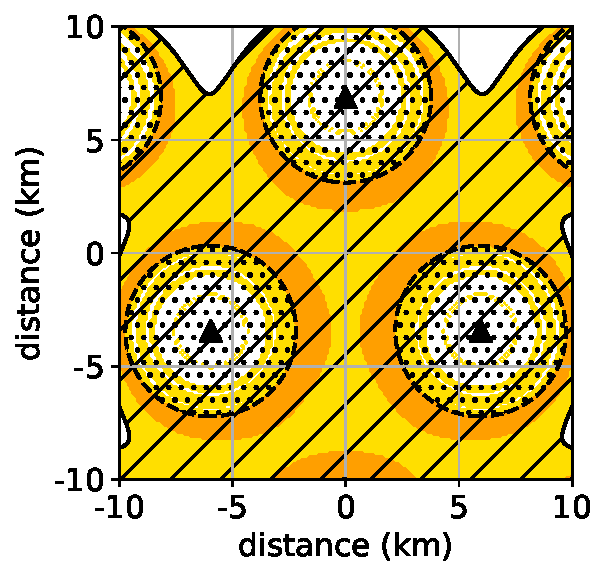
\includegraphics[height=3.25cm]{figures/sparse_IncreaseHeatmap}
\label{fig:sparse-improvement}}
\hfill
\subfloat[Random placement]{
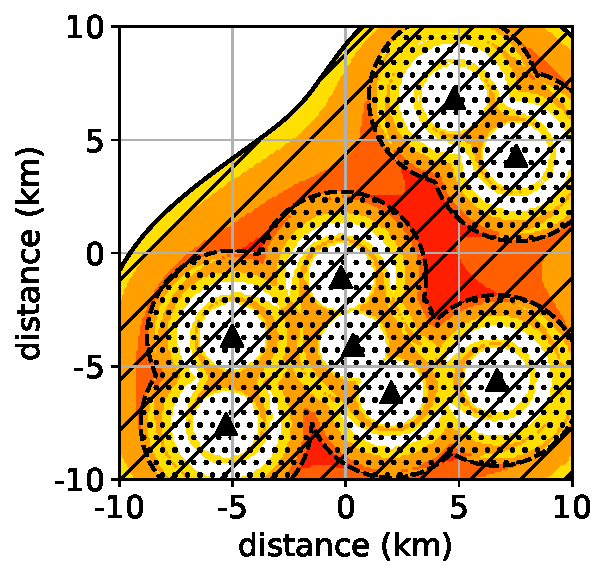
\includegraphics[height=3.25cm]{figures/random_IncreaseHeatmap}
\label{fig:random-improvement}}
\hfill
\subfloat{
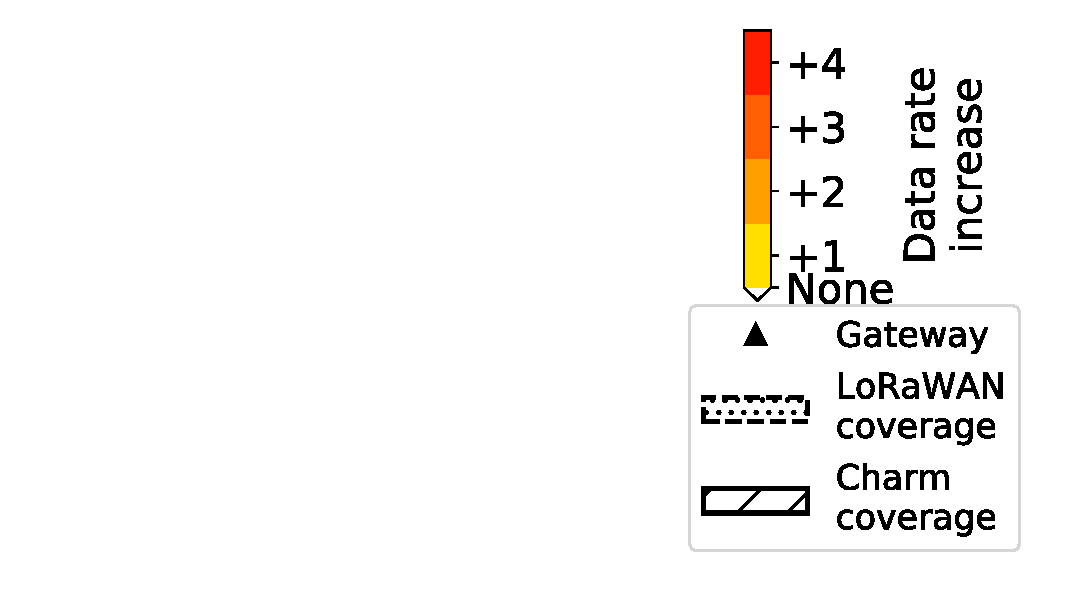
\includegraphics[height=3.25cm]{figures/heatmapLegend}}
\hfill
\setcounter{subfigure}{3}% to se counter to (d) due to skipped caption above
\subfloat[Summary of trace-driven simulations]
\begin{tabular}[b]{r|c|c|c|}
\cline{2-4}
\multicolumn{1}{l|}{} & \begin{tabular}[c]{@{}c@{}}dense\\ cells\end{tabular} & \begin{tabular}[c]{@{}c@{}}sparse\\ cells\end{tabular} & random \\ \hline
\multicolumn{1}{|r|}{\begin{tabular}[c]{@{}r@{}}increase in \\ coverage\end{tabular}} & 46.60\% & 97.85\% & 74.59\% \\ \hline
\multicolumn{1}{|r|}{\begin{tabular}[c]{@{}r@{}}data rate +1\\ (energy/2)\end{tabular}} & 35.33\% & 38.82\% & 33.70\% \\ \hline
\multicolumn{1}{|r|}{\begin{tabular}[c]{@{}r@{}}data rate +2\\ (energy/4)\end{tabular}} & 22.30\% & 0\% & 25.82\% \\ \hline
\multicolumn{1}{|r|}{\begin{tabular}[c]{@{}r@{}}data rate +3\\ (energy/8)\end{tabular}} & 2.26\% & 0\% & 3.48\% \\ \hline
\end{tabular}%
}
\label{table:charm-improvements}
}
\vspace{-10pt}
\caption{Improvement in coverage area and data rates due to Charm.}
\label{fig:charm-improvement}
\compactimg
\end{figure*}

In typical urban settings, users would deploy large number of LoRaWAN
gateways. Indoor settings reduce the range of a LoRaWAN device and the data
rate it can support even for short distances of tens of meters. We deploy
Charm in a congested urban building and demonstrate that collaboration can
improve the maximum range the LoRa device can support at any given data rate.

In this test, we compare a group of regular LoRaWAN gateways that
independently decode transmissions against Charm coherently combining signals
from an ensemble of 4 and 8 gateways. The distances reported in each case are
between the transmitter and the closest gateway. Our results are shown in
Table~\ref{tab:range}. Note that the ranges we observe here are smaller than
outdoor gateways, owing to attenuation inside buildings and transmission power
limits on small portable battery-powered devices. In this context, a regular
LoRaWAN gateway can service client up to approximately 60~m away. In contrast,
Charm consistently supports higher maximum range at each spreading factor. The
results with Charm using eight collaborating gateways show a marked
improvement in range of 200 m, higher than 4 collaborating gateways at 100 m.


\subsection{Effect on coverage and client data rates}
\label{sec:coverage-data-rate-improvement}

In this section, we use trace-driven simulations to show the advantages of
Charm in improving coverage area and client energy consumption in both planned
and unplanned gateway deployments. The signal power at any given receiver is
estimated using the log-distance path loss model. The model is calibrated
using 4850 points collected in a varied urban environment at different data
rates and spreading factors using GPS-connected LoRa client devices. The
log-distance parameters are $L_0  = 98.0729 dB$ for $d_0 = 40.0 m$, $\gamma =
2.1495$ and flat fading $\sigma^2 = 100.0724$. Sensitivity values for the
gateway are taken from \cite{Bor2016} to determine the SNR threshold required
to decode a transmission. In an urban environment with many obstacles and
reflectors, we observe a maximum range of 3.77 km with a transmit power of 15
dBm as opposed to the marketed range of 10 km with line-of-sight. As we are
interested in the trend of changes, we provide an optimistic estimate and
ignore the effects of fading in the simulation (assume $\sigma^2 = 0$).

Assuming the same transmit power on the client of 15 dBm,
\figref{charm-improvement} shows the region where Charm's local detection
followed by joint decoding shows an improvement in either coverage, client
data rates or both compared to independent decoding on gateways (as is
currently done in LoRaWAN). 
The dotted regions show regions which are covered by regular LoRaWAN while the
hatched regions are covered by Charm. Imagine the regions with no coverage
with LoRaWAN having a data rate of DR``-1'' = 0 bps (the next data rate is DR0
= 960 bps using SF = 12). The colored patches are regions where Charm shows an
increase in data rates, with the darker red areas showing larger improvements
than the lighter yellow areas. As seen in each of the sub-figures, Charm shows
an improvement in the coverage area (hatched regions are larger than the
dotted regions), an increase in client data rates (colored ares present inside
the dotted regions) as well as both simultaneously (colored areas outside
LoRaWAN's dotted coverage area). A summary of these results is shown in
Table~\ref{table:charm-improvements}. Every increase in the data rate, doubles
the battery life of a client device. Some regions in the simulation show up to
8 $\times$ energy savings.

\figref{dense-improvement} shows an ideal planned deployment where gateways
are placed in a dense hexagonal grid 6.53 km apart from each other
(corresponding to $2*3.77*\cos(\pi/6)$ km). Such an arrangement, popular in
cellular deployments, provides optimal coverage with no gaps when using an
independent decoding scheme. However, the points farthest from the gateways
(e.g. on the centroid between three neighbouring gateways) have to use the
slowest data rates (corresponding to SF12) and their battery life
correspondingly suffers. If such a deployment were to be augmented with Charm,
the region between the gateways can all communicate using SF9 or better. For
the centroid points, this reduces the transmit time by approximately a factor
of 8 and leads to huge energy savings. Additionally, we see the coverage area
for joint decoding has expanded beyond the original coverage region. Some of
the devices in the expanded coverage area can even communicate with higher
data rates.
An interesting phenomenon seen in each of the sub-figures are the
thin concentric circles of improvement around each gateway. These are regions
just outside the original boundaries covered by any given spreading factor
that also gain a data rate increase due to joint decoding. However, this
effect is not as prominent and the circles are small.

\figref{sparse-improvement} shows a sparse cellular arrangement with gateways
10.05 km apart from each other that can provide gap-free coverage. Charm thus
enables decreasing the gateway density by a factor of 3.33 (proportional to
square of inter-gateway distance $=(11.92/6.53)^2$) while providing the same
level of coverage. Finally, we show in \figref{random-improvement} how Charm
also improves the performance of an unplanned deployment of user-deployed
gateways by improving coverage area as well as data rates for clients. Another
interesting phenomenon to observe here is that Charm's joint decoding manages
to fill in islands and orphaned regions. This is particularly relevant to
urban regions where areas of bad coverage are formed in building basements and
other indoor regions as seen in \figref{penetration-test}.